\documentclass{article}
\usepackage{tikz}
\usetikzlibrary{matrix}
\usepackage[margin=1in]{geometry}
\begin{document}
% --- Frame 0 ---
\begin{center}\LARGE\textbf{DFS}\\[6mm]\end{center}
\begin{center}
\begin{flushleft}\textbf{Log}\\[1.75mm]\end{flushleft}

\begin{tikzpicture}
  \filldraw[fill=white!0, draw=none] (0,0) rectangle (10cm, -0.25cm);
  \node[anchor=north, align=center, text=black] at (5cm,0) {\texttt{Popping last node from stack}};
\end{tikzpicture}
\end{center}
\noindent\rule{\linewidth}{0.3pt}
\begin{center}
\begin{flushleft}\textbf{Graph}\\[2mm]\end{flushleft}
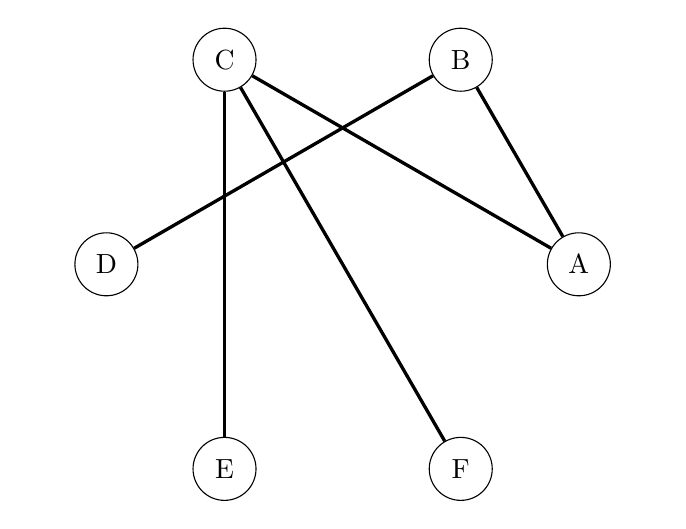
\begin{tikzpicture}
  \filldraw[fill=white!0, draw=none] (-4cm,0) rectangle (4cm, -3cm);
  \node[circle, draw, minimum size=8mm, fill=white] (A) at (0.0:3cm) {A};
  \node[circle, draw, minimum size=8mm, fill=white] (B) at (60.0:3cm) {B};
  \node[circle, draw, minimum size=8mm, fill=white] (C) at (120.0:3cm) {C};
  \node[circle, draw, minimum size=8mm, fill=white] (D) at (180.0:3cm) {D};
  \node[circle, draw, minimum size=8mm, fill=white] (E) at (240.0:3cm) {E};
  \node[circle, draw, minimum size=8mm, fill=white] (F) at (300.0:3cm) {F};
  \draw[black, line width=1.2pt] (A) -- (B);
  \draw[black, line width=1.2pt] (A) -- (C);
  \draw[black, line width=1.2pt] (B) -- (D);
  \draw[black, line width=1.2pt] (C) -- (E);
  \draw[black, line width=1.2pt] (C) -- (F);
\end{tikzpicture}
\end{center}
\noindent\rule{\linewidth}{0.3pt}
\begin{center}
\begin{flushleft}\textbf{Stack}\\[1.75mm]\end{flushleft}
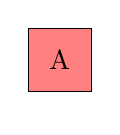
\begin{tikzpicture}
  \filldraw[fill=white!0, draw=none] (0cm,0cm) rectangle (0.8cm, -1cm);
  \filldraw[fill=red!50] (0cm,-0.8cm) rectangle (0.8cm,0cm);
  \node at (0.4cm,-0.4cm) {A};
\end{tikzpicture}
\end{center}
\newpage
% --- Frame 1 ---
\begin{center}\LARGE\textbf{DFS}\\[6mm]\end{center}
\begin{center}
\begin{flushleft}\textbf{Log}\\[1.75mm]\end{flushleft}
\begin{tikzpicture}
  \filldraw[fill=white!0, draw=none] (0,0) rectangle (10cm, -0.25cm);
  \node[anchor=north, align=center, text=black] at (5cm,0) {\texttt{Visiting node A.}};
\end{tikzpicture}
\end{center}
\noindent\rule{\linewidth}{0.3pt}
\begin{center}
\begin{flushleft}\textbf{Graph}\\[2mm]\end{flushleft}
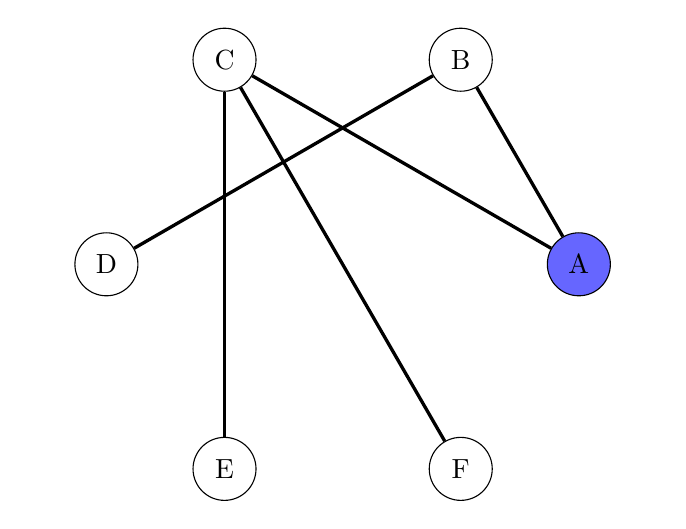
\begin{tikzpicture}
  \filldraw[fill=white!0, draw=none] (-4cm,0) rectangle (4cm, -3cm);
  \node[circle, draw, minimum size=8mm, fill=blue!60] (A) at (0.0:3cm) {A};
  \node[circle, draw, minimum size=8mm, fill=white] (B) at (60.0:3cm) {B};
  \node[circle, draw, minimum size=8mm, fill=white] (C) at (120.0:3cm) {C};
  \node[circle, draw, minimum size=8mm, fill=white] (D) at (180.0:3cm) {D};
  \node[circle, draw, minimum size=8mm, fill=white] (E) at (240.0:3cm) {E};
  \node[circle, draw, minimum size=8mm, fill=white] (F) at (300.0:3cm) {F};
  \draw[black, line width=1.2pt] (A) -- (B);
  \draw[black, line width=1.2pt] (A) -- (C);
  \draw[black, line width=1.2pt] (B) -- (D);
  \draw[black, line width=1.2pt] (C) -- (E);
  \draw[black, line width=1.2pt] (C) -- (F);
\end{tikzpicture}
\end{center}
\noindent\rule{\linewidth}{0.3pt}
\begin{center}
\begin{flushleft}\textbf{Stack}\\[1.75mm]\end{flushleft}
\begin{tikzpicture}
  \filldraw[fill=white!0, draw=none] (0cm,0cm) rectangle (0cm, -1cm);
\end{tikzpicture}
\end{center}
\newpage
% --- Frame 2 ---
\begin{center}\LARGE\textbf{DFS}\\[6mm]\end{center}
\begin{center}
\begin{flushleft}\textbf{Log}\\[1.75mm]\end{flushleft}

\begin{tikzpicture}
  \filldraw[fill=white!0, draw=none] (0,0) rectangle (10cm, -0.25cm);
  \node[anchor=north, align=center, text=black] at (5cm,0) {\texttt{Adding node A's neighbors to stack.}};
\end{tikzpicture}
\end{center}
\noindent\rule{\linewidth}{0.3pt}
\begin{center}
\begin{flushleft}\textbf{Graph}\\[2mm]\end{flushleft}
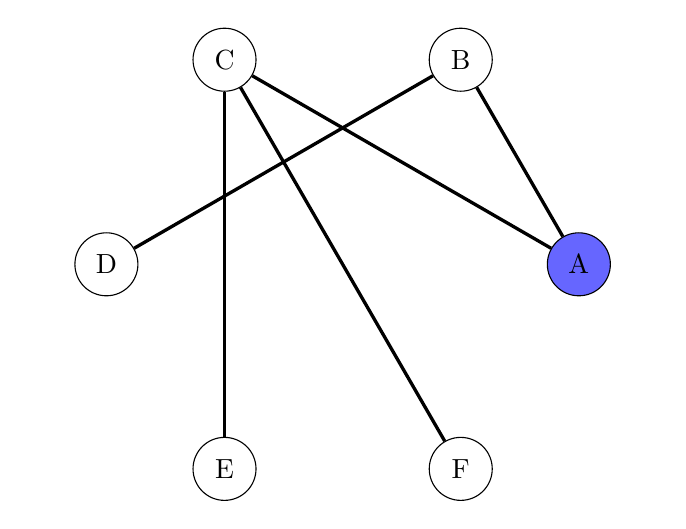
\begin{tikzpicture}
  \filldraw[fill=white!0, draw=none] (-4cm,0) rectangle (4cm, -3cm);
  \node[circle, draw, minimum size=8mm, fill=blue!60] (A) at (0.0:3cm) {A};
  \node[circle, draw, minimum size=8mm, fill=white] (B) at (60.0:3cm) {B};
  \node[circle, draw, minimum size=8mm, fill=white] (C) at (120.0:3cm) {C};
  \node[circle, draw, minimum size=8mm, fill=white] (D) at (180.0:3cm) {D};
  \node[circle, draw, minimum size=8mm, fill=white] (E) at (240.0:3cm) {E};
  \node[circle, draw, minimum size=8mm, fill=white] (F) at (300.0:3cm) {F};
  \draw[black, line width=1.2pt] (A) -- (B);
  \draw[black, line width=1.2pt] (A) -- (C);
  \draw[black, line width=1.2pt] (B) -- (D);
  \draw[black, line width=1.2pt] (C) -- (E);
  \draw[black, line width=1.2pt] (C) -- (F);
\end{tikzpicture}
\end{center}
\noindent\rule{\linewidth}{0.3pt}
\begin{center}
\begin{flushleft}\textbf{Stack}\\[1.75mm]\end{flushleft}
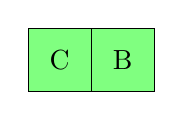
\begin{tikzpicture}
  \filldraw[fill=white!0, draw=none] (0cm,0cm) rectangle (1.6cm, -1cm);
  \filldraw[fill=green!50] (0cm,-0.8cm) rectangle (0.8cm,0cm);
  \node at (0.4cm,-0.4cm) {C};
  \filldraw[fill=green!50] (0.8cm,-0.8cm) rectangle (1.6cm,0cm);
  \node at (1.2000000000000002cm,-0.4cm) {B};
\end{tikzpicture}
\end{center}
\newpage
% --- Frame 3 ---
\begin{center}\LARGE\textbf{DFS}\\[6mm]\end{center}
\begin{center}
\begin{flushleft}\textbf{Log}\\[1.75mm]\end{flushleft}

\begin{tikzpicture}
  \filldraw[fill=white!0, draw=none] (0,0) rectangle (10cm, -0.25cm);
  \node[anchor=north, align=center, text=black] at (5cm,0) {\texttt{Popping last node from stack}};
\end{tikzpicture}
\end{center}
\noindent\rule{\linewidth}{0.3pt}
\begin{center}
\begin{flushleft}\textbf{Graph}\\[2mm]\end{flushleft}
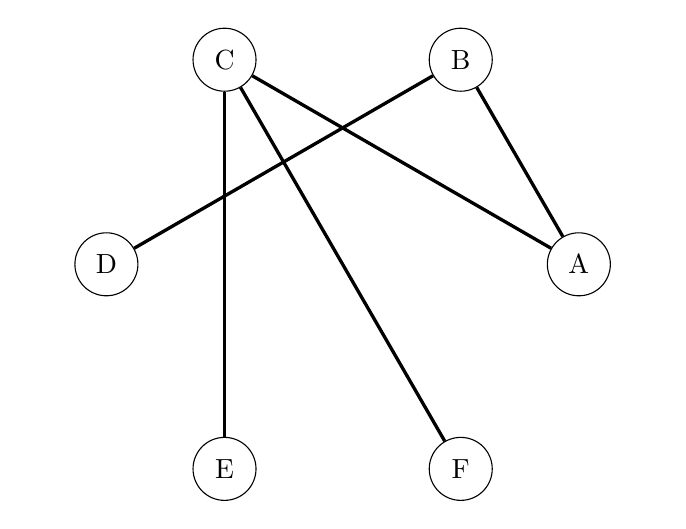
\begin{tikzpicture}
  \filldraw[fill=white!0, draw=none] (-4cm,0) rectangle (4cm, -3cm);
  \node[circle, draw, minimum size=8mm, fill=white] (A) at (0.0:3cm) {A};
  \node[circle, draw, minimum size=8mm, fill=white] (B) at (60.0:3cm) {B};
  \node[circle, draw, minimum size=8mm, fill=white] (C) at (120.0:3cm) {C};
  \node[circle, draw, minimum size=8mm, fill=white] (D) at (180.0:3cm) {D};
  \node[circle, draw, minimum size=8mm, fill=white] (E) at (240.0:3cm) {E};
  \node[circle, draw, minimum size=8mm, fill=white] (F) at (300.0:3cm) {F};
  \draw[black, line width=1.2pt] (A) -- (B);
  \draw[black, line width=1.2pt] (A) -- (C);
  \draw[black, line width=1.2pt] (B) -- (D);
  \draw[black, line width=1.2pt] (C) -- (E);
  \draw[black, line width=1.2pt] (C) -- (F);
\end{tikzpicture}
\end{center}
\noindent\rule{\linewidth}{0.3pt}
\begin{center}
\begin{flushleft}\textbf{Stack}\\[1.75mm]\end{flushleft}
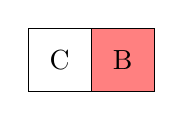
\begin{tikzpicture}
  \filldraw[fill=white!0, draw=none] (0cm,0cm) rectangle (1.6cm, -1cm);
  \filldraw[fill=white] (0cm,-0.8cm) rectangle (0.8cm,0cm);
  \node at (0.4cm,-0.4cm) {C};
  \filldraw[fill=red!50] (0.8cm,-0.8cm) rectangle (1.6cm,0cm);
  \node at (1.2000000000000002cm,-0.4cm) {B};
\end{tikzpicture}
\end{center}
\newpage
% --- Frame 4 ---
\begin{center}\LARGE\textbf{DFS}\\[6mm]\end{center}
\begin{center}
\begin{flushleft}\textbf{Log}\\[1.75mm]\end{flushleft}
\begin{tikzpicture}
  \filldraw[fill=white!0, draw=none] (0,0) rectangle (10cm, -0.25cm);
  \node[anchor=north, align=center, text=black] at (5cm,0) {\texttt{Visiting node B.}};
\end{tikzpicture}
\end{center}
\noindent\rule{\linewidth}{0.3pt}
\begin{center}
\begin{flushleft}\textbf{Graph}\\[2mm]\end{flushleft}
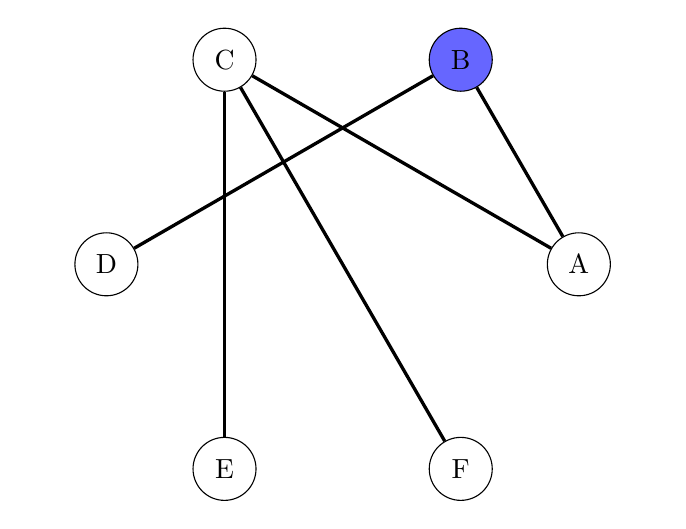
\begin{tikzpicture}
  \filldraw[fill=white!0, draw=none] (-4cm,0) rectangle (4cm, -3cm);
  \node[circle, draw, minimum size=8mm, fill=white] (A) at (0.0:3cm) {A};
  \node[circle, draw, minimum size=8mm, fill=blue!60] (B) at (60.0:3cm) {B};
  \node[circle, draw, minimum size=8mm, fill=white] (C) at (120.0:3cm) {C};
  \node[circle, draw, minimum size=8mm, fill=white] (D) at (180.0:3cm) {D};
  \node[circle, draw, minimum size=8mm, fill=white] (E) at (240.0:3cm) {E};
  \node[circle, draw, minimum size=8mm, fill=white] (F) at (300.0:3cm) {F};
  \draw[black, line width=1.2pt] (A) -- (B);
  \draw[black, line width=1.2pt] (A) -- (C);
  \draw[black, line width=1.2pt] (B) -- (D);
  \draw[black, line width=1.2pt] (C) -- (E);
  \draw[black, line width=1.2pt] (C) -- (F);
\end{tikzpicture}
\end{center}
\noindent\rule{\linewidth}{0.3pt}
\begin{center}
\begin{flushleft}\textbf{Stack}\\[1.75mm]\end{flushleft}
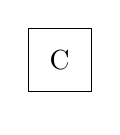
\begin{tikzpicture}
  \filldraw[fill=white!0, draw=none] (0cm,0cm) rectangle (0.8cm, -1cm);
  \filldraw[fill=white] (0cm,-0.8cm) rectangle (0.8cm,0cm);
  \node at (0.4cm,-0.4cm) {C};
\end{tikzpicture}
\end{center}
\newpage
% --- Frame 5 ---
\begin{center}\LARGE\textbf{DFS}\\[6mm]\end{center}
\begin{center}
\begin{flushleft}\textbf{Log}\\[1.75mm]\end{flushleft}

\begin{tikzpicture}
  \filldraw[fill=white!0, draw=none] (0,0) rectangle (10cm, -0.25cm);
  \node[anchor=north, align=center, text=black] at (5cm,0) {\texttt{Adding node B's neighbors to stack.}};
\end{tikzpicture}
\end{center}
\noindent\rule{\linewidth}{0.3pt}
\begin{center}
\begin{flushleft}\textbf{Graph}\\[2mm]\end{flushleft}
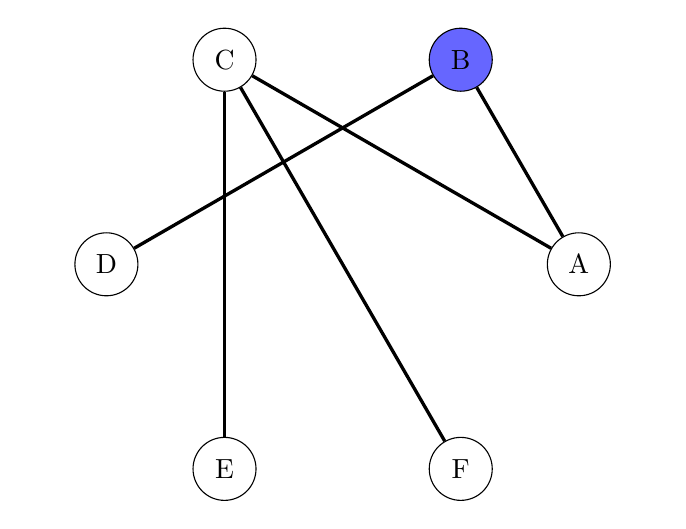
\begin{tikzpicture}
  \filldraw[fill=white!0, draw=none] (-4cm,0) rectangle (4cm, -3cm);
  \node[circle, draw, minimum size=8mm, fill=white] (A) at (0.0:3cm) {A};
  \node[circle, draw, minimum size=8mm, fill=blue!60] (B) at (60.0:3cm) {B};
  \node[circle, draw, minimum size=8mm, fill=white] (C) at (120.0:3cm) {C};
  \node[circle, draw, minimum size=8mm, fill=white] (D) at (180.0:3cm) {D};
  \node[circle, draw, minimum size=8mm, fill=white] (E) at (240.0:3cm) {E};
  \node[circle, draw, minimum size=8mm, fill=white] (F) at (300.0:3cm) {F};
  \draw[black, line width=1.2pt] (A) -- (B);
  \draw[black, line width=1.2pt] (A) -- (C);
  \draw[black, line width=1.2pt] (B) -- (D);
  \draw[black, line width=1.2pt] (C) -- (E);
  \draw[black, line width=1.2pt] (C) -- (F);
\end{tikzpicture}
\end{center}
\noindent\rule{\linewidth}{0.3pt}
\begin{center}
\begin{flushleft}\textbf{Stack}\\[1.75mm]\end{flushleft}
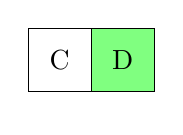
\begin{tikzpicture}
  \filldraw[fill=white!0, draw=none] (0cm,0cm) rectangle (1.6cm, -1cm);
  \filldraw[fill=white] (0cm,-0.8cm) rectangle (0.8cm,0cm);
  \node at (0.4cm,-0.4cm) {C};
  \filldraw[fill=green!50] (0.8cm,-0.8cm) rectangle (1.6cm,0cm);
  \node at (1.2000000000000002cm,-0.4cm) {D};
\end{tikzpicture}
\end{center}
\newpage
% --- Frame 6 ---
\begin{center}\LARGE\textbf{DFS}\\[6mm]\end{center}
\begin{center}
\begin{flushleft}\textbf{Log}\\[1.75mm]\end{flushleft}

\begin{tikzpicture}
  \filldraw[fill=white!0, draw=none] (0,0) rectangle (10cm, -0.25cm);
  \node[anchor=north, align=center, text=black] at (5cm,0) {\texttt{Popping last node from stack}};
\end{tikzpicture}
\end{center}
\noindent\rule{\linewidth}{0.3pt}
\begin{center}
\begin{flushleft}\textbf{Graph}\\[2mm]\end{flushleft}
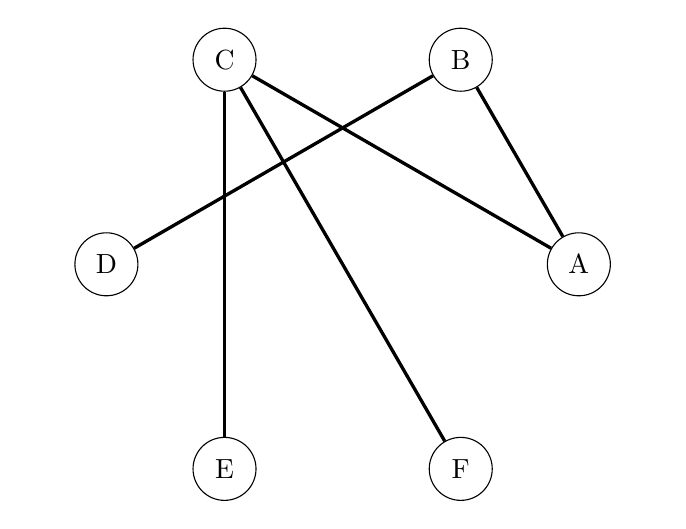
\begin{tikzpicture}
  \filldraw[fill=white!0, draw=none] (-4cm,0) rectangle (4cm, -3cm);
  \node[circle, draw, minimum size=8mm, fill=white] (A) at (0.0:3cm) {A};
  \node[circle, draw, minimum size=8mm, fill=white] (B) at (60.0:3cm) {B};
  \node[circle, draw, minimum size=8mm, fill=white] (C) at (120.0:3cm) {C};
  \node[circle, draw, minimum size=8mm, fill=white] (D) at (180.0:3cm) {D};
  \node[circle, draw, minimum size=8mm, fill=white] (E) at (240.0:3cm) {E};
  \node[circle, draw, minimum size=8mm, fill=white] (F) at (300.0:3cm) {F};
  \draw[black, line width=1.2pt] (A) -- (B);
  \draw[black, line width=1.2pt] (A) -- (C);
  \draw[black, line width=1.2pt] (B) -- (D);
  \draw[black, line width=1.2pt] (C) -- (E);
  \draw[black, line width=1.2pt] (C) -- (F);
\end{tikzpicture}
\end{center}
\noindent\rule{\linewidth}{0.3pt}
\begin{center}
\begin{flushleft}\textbf{Stack}\\[1.75mm]\end{flushleft}
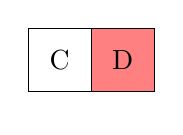
\begin{tikzpicture}
  \filldraw[fill=white!0, draw=none] (0cm,0cm) rectangle (1.6cm, -1cm);
  \filldraw[fill=white] (0cm,-0.8cm) rectangle (0.8cm,0cm);
  \node at (0.4cm,-0.4cm) {C};
  \filldraw[fill=red!50] (0.8cm,-0.8cm) rectangle (1.6cm,0cm);
  \node at (1.2000000000000002cm,-0.4cm) {D};
\end{tikzpicture}
\end{center}
\newpage
% --- Frame 7 ---
\begin{center}\LARGE\textbf{DFS}\\[6mm]\end{center}
\begin{center}
\begin{flushleft}\textbf{Log}\\[1.75mm]\end{flushleft}
\begin{tikzpicture}
  \filldraw[fill=white!0, draw=none] (0,0) rectangle (10cm, -0.25cm);
  \node[anchor=north, align=center, text=black] at (5cm,0) {\texttt{Visiting node D.}};
\end{tikzpicture}
\end{center}
\noindent\rule{\linewidth}{0.3pt}
\begin{center}
\begin{flushleft}\textbf{Graph}\\[2mm]\end{flushleft}
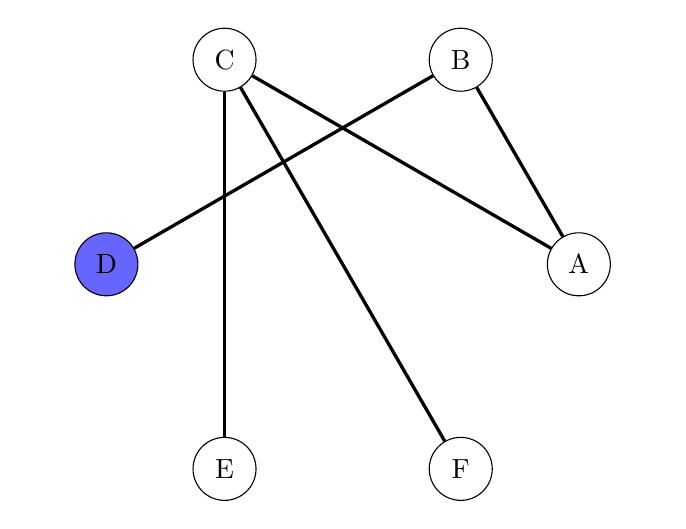
\begin{tikzpicture}
  \filldraw[fill=white!0, draw=none] (-4cm,0) rectangle (4cm, -3cm);
  \node[circle, draw, minimum size=8mm, fill=white] (A) at (0.0:3cm) {A};
  \node[circle, draw, minimum size=8mm, fill=white] (B) at (60.0:3cm) {B};
  \node[circle, draw, minimum size=8mm, fill=white] (C) at (120.0:3cm) {C};
  \node[circle, draw, minimum size=8mm, fill=blue!60] (D) at (180.0:3cm) {D};
  \node[circle, draw, minimum size=8mm, fill=white] (E) at (240.0:3cm) {E};
  \node[circle, draw, minimum size=8mm, fill=white] (F) at (300.0:3cm) {F};
  \draw[black, line width=1.2pt] (A) -- (B);
  \draw[black, line width=1.2pt] (A) -- (C);
  \draw[black, line width=1.2pt] (B) -- (D);
  \draw[black, line width=1.2pt] (C) -- (E);
  \draw[black, line width=1.2pt] (C) -- (F);
\end{tikzpicture}
\end{center}
\noindent\rule{\linewidth}{0.3pt}
\begin{center}
\begin{flushleft}\textbf{Stack}\\[1.75mm]\end{flushleft}
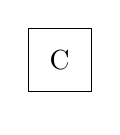
\begin{tikzpicture}
  \filldraw[fill=white!0, draw=none] (0cm,0cm) rectangle (0.8cm, -1cm);
  \filldraw[fill=white] (0cm,-0.8cm) rectangle (0.8cm,0cm);
  \node at (0.4cm,-0.4cm) {C};
\end{tikzpicture}
\end{center}
\newpage
% --- Frame 8 ---
\begin{center}\LARGE\textbf{DFS}\\[6mm]\end{center}
\begin{center}
\begin{flushleft}\textbf{Log}\\[1.75mm]\end{flushleft}

\begin{tikzpicture}
  \filldraw[fill=white!0, draw=none] (0,0) rectangle (10cm, -0.25cm);
  \node[anchor=north, align=center, text=black] at (5cm,0) {\texttt{Adding node D's neighbors to stack.}};
\end{tikzpicture}
\end{center}
\noindent\rule{\linewidth}{0.3pt}
\begin{center}
\begin{flushleft}\textbf{Graph}\\[2mm]\end{flushleft}
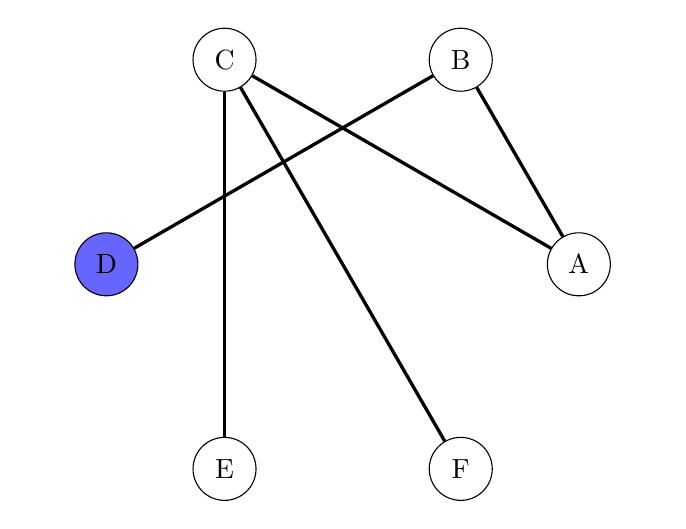
\begin{tikzpicture}
  \filldraw[fill=white!0, draw=none] (-4cm,0) rectangle (4cm, -3cm);
  \node[circle, draw, minimum size=8mm, fill=white] (A) at (0.0:3cm) {A};
  \node[circle, draw, minimum size=8mm, fill=white] (B) at (60.0:3cm) {B};
  \node[circle, draw, minimum size=8mm, fill=white] (C) at (120.0:3cm) {C};
  \node[circle, draw, minimum size=8mm, fill=blue!60] (D) at (180.0:3cm) {D};
  \node[circle, draw, minimum size=8mm, fill=white] (E) at (240.0:3cm) {E};
  \node[circle, draw, minimum size=8mm, fill=white] (F) at (300.0:3cm) {F};
  \draw[black, line width=1.2pt] (A) -- (B);
  \draw[black, line width=1.2pt] (A) -- (C);
  \draw[black, line width=1.2pt] (B) -- (D);
  \draw[black, line width=1.2pt] (C) -- (E);
  \draw[black, line width=1.2pt] (C) -- (F);
\end{tikzpicture}
\end{center}
\noindent\rule{\linewidth}{0.3pt}
\begin{center}
\begin{flushleft}\textbf{Stack}\\[1.75mm]\end{flushleft}
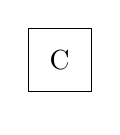
\begin{tikzpicture}
  \filldraw[fill=white!0, draw=none] (0cm,0cm) rectangle (0.8cm, -1cm);
  \filldraw[fill=white] (0cm,-0.8cm) rectangle (0.8cm,0cm);
  \node at (0.4cm,-0.4cm) {C};
\end{tikzpicture}
\end{center}
\newpage
% --- Frame 9 ---
\begin{center}\LARGE\textbf{DFS}\\[6mm]\end{center}
\begin{center}
\begin{flushleft}\textbf{Log}\\[1.75mm]\end{flushleft}

\begin{tikzpicture}
  \filldraw[fill=white!0, draw=none] (0,0) rectangle (10cm, -0.25cm);
  \node[anchor=north, align=center, text=black] at (5cm,0) {\texttt{Popping last node from stack}};
\end{tikzpicture}
\end{center}
\noindent\rule{\linewidth}{0.3pt}
\begin{center}
\begin{flushleft}\textbf{Graph}\\[2mm]\end{flushleft}
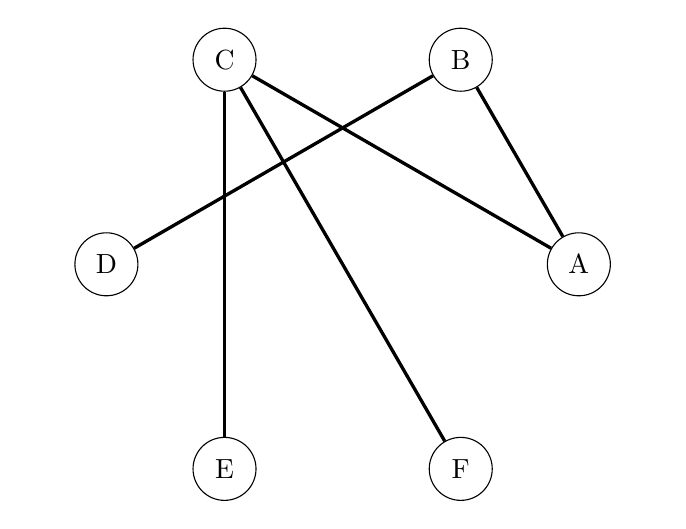
\begin{tikzpicture}
  \filldraw[fill=white!0, draw=none] (-4cm,0) rectangle (4cm, -3cm);
  \node[circle, draw, minimum size=8mm, fill=white] (A) at (0.0:3cm) {A};
  \node[circle, draw, minimum size=8mm, fill=white] (B) at (60.0:3cm) {B};
  \node[circle, draw, minimum size=8mm, fill=white] (C) at (120.0:3cm) {C};
  \node[circle, draw, minimum size=8mm, fill=white] (D) at (180.0:3cm) {D};
  \node[circle, draw, minimum size=8mm, fill=white] (E) at (240.0:3cm) {E};
  \node[circle, draw, minimum size=8mm, fill=white] (F) at (300.0:3cm) {F};
  \draw[black, line width=1.2pt] (A) -- (B);
  \draw[black, line width=1.2pt] (A) -- (C);
  \draw[black, line width=1.2pt] (B) -- (D);
  \draw[black, line width=1.2pt] (C) -- (E);
  \draw[black, line width=1.2pt] (C) -- (F);
\end{tikzpicture}
\end{center}
\noindent\rule{\linewidth}{0.3pt}
\begin{center}
\begin{flushleft}\textbf{Stack}\\[1.75mm]\end{flushleft}
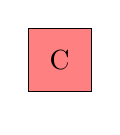
\begin{tikzpicture}
  \filldraw[fill=white!0, draw=none] (0cm,0cm) rectangle (0.8cm, -1cm);
  \filldraw[fill=red!50] (0cm,-0.8cm) rectangle (0.8cm,0cm);
  \node at (0.4cm,-0.4cm) {C};
\end{tikzpicture}
\end{center}
\newpage
% --- Frame 10 ---
\begin{center}\LARGE\textbf{DFS}\\[6mm]\end{center}
\begin{center}
\begin{flushleft}\textbf{Log}\\[1.75mm]\end{flushleft}
\begin{tikzpicture}
  \filldraw[fill=white!0, draw=none] (0,0) rectangle (10cm, -0.25cm);
  \node[anchor=north, align=center, text=black] at (5cm,0) {\texttt{Visiting node C.}};
\end{tikzpicture}
\end{center}
\noindent\rule{\linewidth}{0.3pt}
\begin{center}
\begin{flushleft}\textbf{Graph}\\[2mm]\end{flushleft}
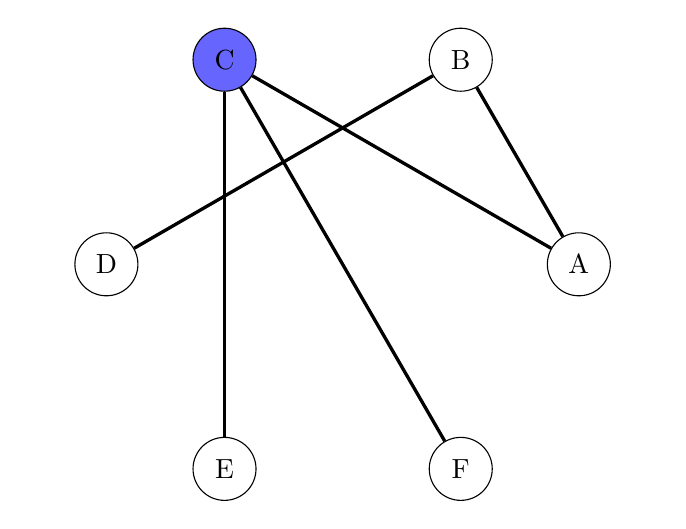
\begin{tikzpicture}
  \filldraw[fill=white!0, draw=none] (-4cm,0) rectangle (4cm, -3cm);
  \node[circle, draw, minimum size=8mm, fill=white] (A) at (0.0:3cm) {A};
  \node[circle, draw, minimum size=8mm, fill=white] (B) at (60.0:3cm) {B};
  \node[circle, draw, minimum size=8mm, fill=blue!60] (C) at (120.0:3cm) {C};
  \node[circle, draw, minimum size=8mm, fill=white] (D) at (180.0:3cm) {D};
  \node[circle, draw, minimum size=8mm, fill=white] (E) at (240.0:3cm) {E};
  \node[circle, draw, minimum size=8mm, fill=white] (F) at (300.0:3cm) {F};
  \draw[black, line width=1.2pt] (A) -- (B);
  \draw[black, line width=1.2pt] (A) -- (C);
  \draw[black, line width=1.2pt] (B) -- (D);
  \draw[black, line width=1.2pt] (C) -- (E);
  \draw[black, line width=1.2pt] (C) -- (F);
\end{tikzpicture}
\end{center}
\noindent\rule{\linewidth}{0.3pt}
\begin{center}
\begin{flushleft}\textbf{Stack}\\[1.75mm]\end{flushleft}
\begin{tikzpicture}
  \filldraw[fill=white!0, draw=none] (0cm,0cm) rectangle (0cm, -1cm);
\end{tikzpicture}
\end{center}
\newpage
% --- Frame 11 ---
\begin{center}\LARGE\textbf{DFS}\\[6mm]\end{center}
\begin{center}
\begin{flushleft}\textbf{Log}\\[1.75mm]\end{flushleft}

\begin{tikzpicture}
  \filldraw[fill=white!0, draw=none] (0,0) rectangle (10cm, -0.25cm);
  \node[anchor=north, align=center, text=black] at (5cm,0) {\texttt{Adding node C's neighbors to stack.}};
\end{tikzpicture}
\end{center}
\noindent\rule{\linewidth}{0.3pt}
\begin{center}
\begin{flushleft}\textbf{Graph}\\[2mm]\end{flushleft}
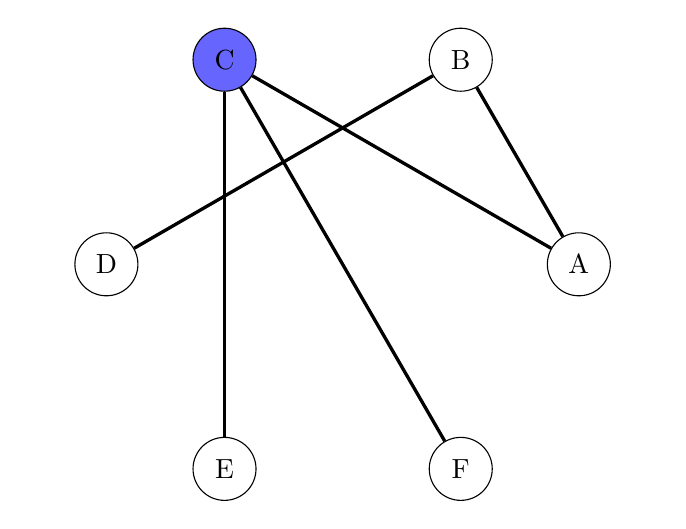
\begin{tikzpicture}
  \filldraw[fill=white!0, draw=none] (-4cm,0) rectangle (4cm, -3cm);
  \node[circle, draw, minimum size=8mm, fill=white] (A) at (0.0:3cm) {A};
  \node[circle, draw, minimum size=8mm, fill=white] (B) at (60.0:3cm) {B};
  \node[circle, draw, minimum size=8mm, fill=blue!60] (C) at (120.0:3cm) {C};
  \node[circle, draw, minimum size=8mm, fill=white] (D) at (180.0:3cm) {D};
  \node[circle, draw, minimum size=8mm, fill=white] (E) at (240.0:3cm) {E};
  \node[circle, draw, minimum size=8mm, fill=white] (F) at (300.0:3cm) {F};
  \draw[black, line width=1.2pt] (A) -- (B);
  \draw[black, line width=1.2pt] (A) -- (C);
  \draw[black, line width=1.2pt] (B) -- (D);
  \draw[black, line width=1.2pt] (C) -- (E);
  \draw[black, line width=1.2pt] (C) -- (F);
\end{tikzpicture}
\end{center}
\noindent\rule{\linewidth}{0.3pt}
\begin{center}
\begin{flushleft}\textbf{Stack}\\[1.75mm]\end{flushleft}
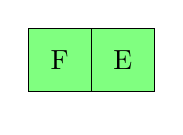
\begin{tikzpicture}
  \filldraw[fill=white!0, draw=none] (0cm,0cm) rectangle (1.6cm, -1cm);
  \filldraw[fill=green!50] (0cm,-0.8cm) rectangle (0.8cm,0cm);
  \node at (0.4cm,-0.4cm) {F};
  \filldraw[fill=green!50] (0.8cm,-0.8cm) rectangle (1.6cm,0cm);
  \node at (1.2000000000000002cm,-0.4cm) {E};
\end{tikzpicture}
\end{center}
\newpage
% --- Frame 12 ---
\begin{center}\LARGE\textbf{DFS}\\[6mm]\end{center}
\begin{center}
\begin{flushleft}\textbf{Log}\\[1.75mm]\end{flushleft}

\begin{tikzpicture}
  \filldraw[fill=white!0, draw=none] (0,0) rectangle (10cm, -0.25cm);
  \node[anchor=north, align=center, text=black] at (5cm,0) {\texttt{Popping last node from stack}};
\end{tikzpicture}
\end{center}
\noindent\rule{\linewidth}{0.3pt}
\begin{center}
\begin{flushleft}\textbf{Graph}\\[2mm]\end{flushleft}
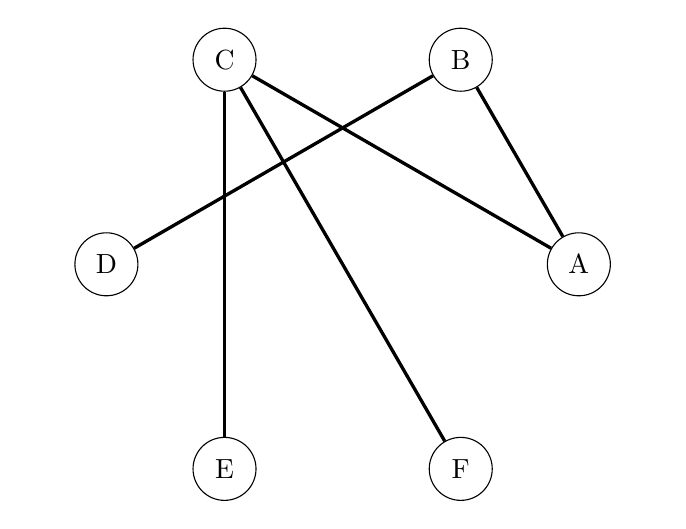
\begin{tikzpicture}
  \filldraw[fill=white!0, draw=none] (-4cm,0) rectangle (4cm, -3cm);
  \node[circle, draw, minimum size=8mm, fill=white] (A) at (0.0:3cm) {A};
  \node[circle, draw, minimum size=8mm, fill=white] (B) at (60.0:3cm) {B};
  \node[circle, draw, minimum size=8mm, fill=white] (C) at (120.0:3cm) {C};
  \node[circle, draw, minimum size=8mm, fill=white] (D) at (180.0:3cm) {D};
  \node[circle, draw, minimum size=8mm, fill=white] (E) at (240.0:3cm) {E};
  \node[circle, draw, minimum size=8mm, fill=white] (F) at (300.0:3cm) {F};
  \draw[black, line width=1.2pt] (A) -- (B);
  \draw[black, line width=1.2pt] (A) -- (C);
  \draw[black, line width=1.2pt] (B) -- (D);
  \draw[black, line width=1.2pt] (C) -- (E);
  \draw[black, line width=1.2pt] (C) -- (F);
\end{tikzpicture}
\end{center}
\noindent\rule{\linewidth}{0.3pt}
\begin{center}
\begin{flushleft}\textbf{Stack}\\[1.75mm]\end{flushleft}
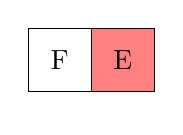
\begin{tikzpicture}
  \filldraw[fill=white!0, draw=none] (0cm,0cm) rectangle (1.6cm, -1cm);
  \filldraw[fill=white] (0cm,-0.8cm) rectangle (0.8cm,0cm);
  \node at (0.4cm,-0.4cm) {F};
  \filldraw[fill=red!50] (0.8cm,-0.8cm) rectangle (1.6cm,0cm);
  \node at (1.2000000000000002cm,-0.4cm) {E};
\end{tikzpicture}
\end{center}
\newpage
% --- Frame 13 ---
\begin{center}\LARGE\textbf{DFS}\\[6mm]\end{center}
\begin{center}
\begin{flushleft}\textbf{Log}\\[1.75mm]\end{flushleft}
\begin{tikzpicture}
  \filldraw[fill=white!0, draw=none] (0,0) rectangle (10cm, -0.25cm);
  \node[anchor=north, align=center, text=black] at (5cm,0) {\texttt{Visiting node E.}};
\end{tikzpicture}
\end{center}
\noindent\rule{\linewidth}{0.3pt}
\begin{center}
\begin{flushleft}\textbf{Graph}\\[2mm]\end{flushleft}
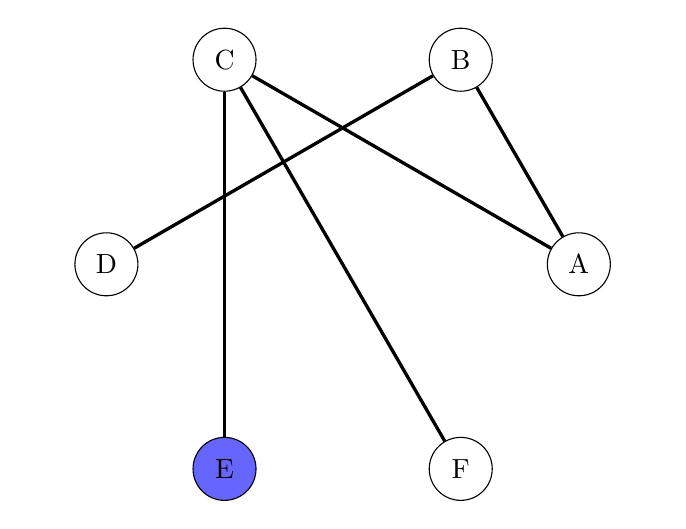
\begin{tikzpicture}
  \filldraw[fill=white!0, draw=none] (-4cm,0) rectangle (4cm, -3cm);
  \node[circle, draw, minimum size=8mm, fill=white] (A) at (0.0:3cm) {A};
  \node[circle, draw, minimum size=8mm, fill=white] (B) at (60.0:3cm) {B};
  \node[circle, draw, minimum size=8mm, fill=white] (C) at (120.0:3cm) {C};
  \node[circle, draw, minimum size=8mm, fill=white] (D) at (180.0:3cm) {D};
  \node[circle, draw, minimum size=8mm, fill=blue!60] (E) at (240.0:3cm) {E};
  \node[circle, draw, minimum size=8mm, fill=white] (F) at (300.0:3cm) {F};
  \draw[black, line width=1.2pt] (A) -- (B);
  \draw[black, line width=1.2pt] (A) -- (C);
  \draw[black, line width=1.2pt] (B) -- (D);
  \draw[black, line width=1.2pt] (C) -- (E);
  \draw[black, line width=1.2pt] (C) -- (F);
\end{tikzpicture}
\end{center}
\noindent\rule{\linewidth}{0.3pt}
\begin{center}
\begin{flushleft}\textbf{Stack}\\[1.75mm]\end{flushleft}
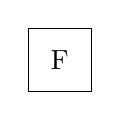
\begin{tikzpicture}
  \filldraw[fill=white!0, draw=none] (0cm,0cm) rectangle (0.8cm, -1cm);
  \filldraw[fill=white] (0cm,-0.8cm) rectangle (0.8cm,0cm);
  \node at (0.4cm,-0.4cm) {F};
\end{tikzpicture}
\end{center}
\newpage
% --- Frame 14 ---
\begin{center}\LARGE\textbf{DFS}\\[6mm]\end{center}
\begin{center}
\begin{flushleft}\textbf{Log}\\[1.75mm]\end{flushleft}

\begin{tikzpicture}
  \filldraw[fill=white!0, draw=none] (0,0) rectangle (10cm, -0.25cm);
  \node[anchor=north, align=center, text=black] at (5cm,0) {\texttt{Adding node E's neighbors to stack.}};
\end{tikzpicture}
\end{center}
\noindent\rule{\linewidth}{0.3pt}
\begin{center}
\begin{flushleft}\textbf{Graph}\\[2mm]\end{flushleft}
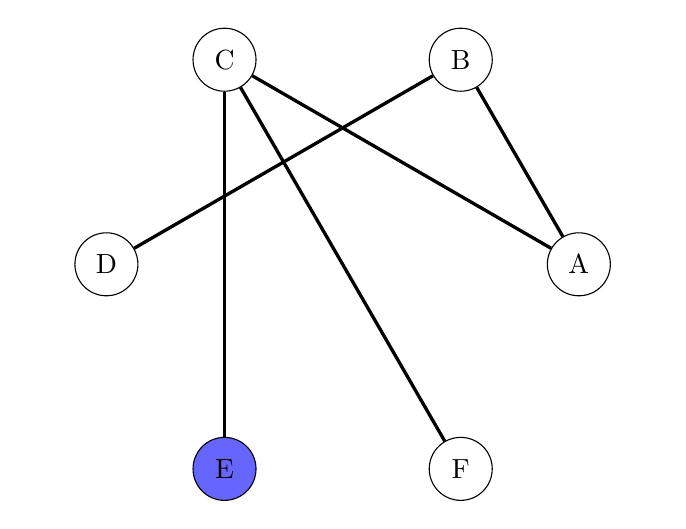
\begin{tikzpicture}
  \filldraw[fill=white!0, draw=none] (-4cm,0) rectangle (4cm, -3cm);
  \node[circle, draw, minimum size=8mm, fill=white] (A) at (0.0:3cm) {A};
  \node[circle, draw, minimum size=8mm, fill=white] (B) at (60.0:3cm) {B};
  \node[circle, draw, minimum size=8mm, fill=white] (C) at (120.0:3cm) {C};
  \node[circle, draw, minimum size=8mm, fill=white] (D) at (180.0:3cm) {D};
  \node[circle, draw, minimum size=8mm, fill=blue!60] (E) at (240.0:3cm) {E};
  \node[circle, draw, minimum size=8mm, fill=white] (F) at (300.0:3cm) {F};
  \draw[black, line width=1.2pt] (A) -- (B);
  \draw[black, line width=1.2pt] (A) -- (C);
  \draw[black, line width=1.2pt] (B) -- (D);
  \draw[black, line width=1.2pt] (C) -- (E);
  \draw[black, line width=1.2pt] (C) -- (F);
\end{tikzpicture}
\end{center}
\noindent\rule{\linewidth}{0.3pt}
\begin{center}
\begin{flushleft}\textbf{Stack}\\[1.75mm]\end{flushleft}
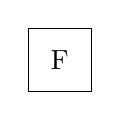
\begin{tikzpicture}
  \filldraw[fill=white!0, draw=none] (0cm,0cm) rectangle (0.8cm, -1cm);
  \filldraw[fill=white] (0cm,-0.8cm) rectangle (0.8cm,0cm);
  \node at (0.4cm,-0.4cm) {F};
\end{tikzpicture}
\end{center}
\newpage
% --- Frame 15 ---
\begin{center}\LARGE\textbf{DFS}\\[6mm]\end{center}
\begin{center}
\begin{flushleft}\textbf{Log}\\[1.75mm]\end{flushleft}

\begin{tikzpicture}
  \filldraw[fill=white!0, draw=none] (0,0) rectangle (10cm, -0.25cm);
  \node[anchor=north, align=center, text=black] at (5cm,0) {\texttt{Popping last node from stack}};
\end{tikzpicture}
\end{center}
\noindent\rule{\linewidth}{0.3pt}
\begin{center}
\begin{flushleft}\textbf{Graph}\\[2mm]\end{flushleft}
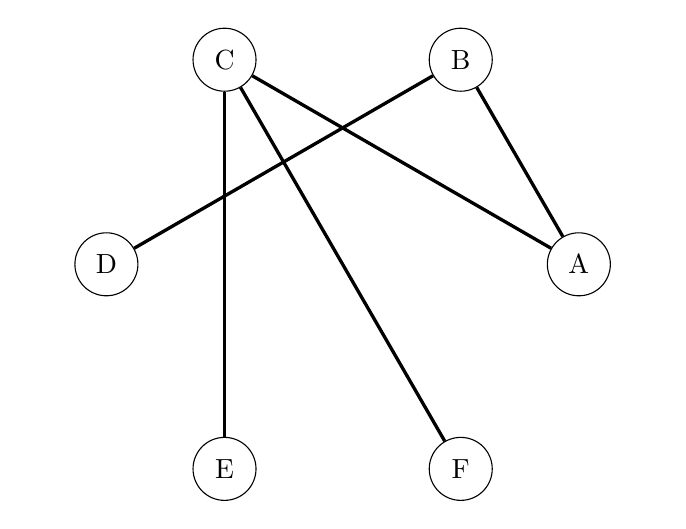
\begin{tikzpicture}
  \filldraw[fill=white!0, draw=none] (-4cm,0) rectangle (4cm, -3cm);
  \node[circle, draw, minimum size=8mm, fill=white] (A) at (0.0:3cm) {A};
  \node[circle, draw, minimum size=8mm, fill=white] (B) at (60.0:3cm) {B};
  \node[circle, draw, minimum size=8mm, fill=white] (C) at (120.0:3cm) {C};
  \node[circle, draw, minimum size=8mm, fill=white] (D) at (180.0:3cm) {D};
  \node[circle, draw, minimum size=8mm, fill=white] (E) at (240.0:3cm) {E};
  \node[circle, draw, minimum size=8mm, fill=white] (F) at (300.0:3cm) {F};
  \draw[black, line width=1.2pt] (A) -- (B);
  \draw[black, line width=1.2pt] (A) -- (C);
  \draw[black, line width=1.2pt] (B) -- (D);
  \draw[black, line width=1.2pt] (C) -- (E);
  \draw[black, line width=1.2pt] (C) -- (F);
\end{tikzpicture}
\end{center}
\noindent\rule{\linewidth}{0.3pt}
\begin{center}
\begin{flushleft}\textbf{Stack}\\[1.75mm]\end{flushleft}
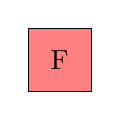
\begin{tikzpicture}
  \filldraw[fill=white!0, draw=none] (0cm,0cm) rectangle (0.8cm, -1cm);
  \filldraw[fill=red!50] (0cm,-0.8cm) rectangle (0.8cm,0cm);
  \node at (0.4cm,-0.4cm) {F};
\end{tikzpicture}
\end{center}
\newpage
% --- Frame 16 ---
\begin{center}\LARGE\textbf{DFS}\\[6mm]\end{center}
\begin{center}
\begin{flushleft}\textbf{Log}\\[1.75mm]\end{flushleft}
\begin{tikzpicture}
  \filldraw[fill=white!0, draw=none] (0,0) rectangle (10cm, -0.25cm);
  \node[anchor=north, align=center, text=black] at (5cm,0) {\texttt{Visiting node F.}};
\end{tikzpicture}
\end{center}
\noindent\rule{\linewidth}{0.3pt}
\begin{center}
\begin{flushleft}\textbf{Graph}\\[2mm]\end{flushleft}
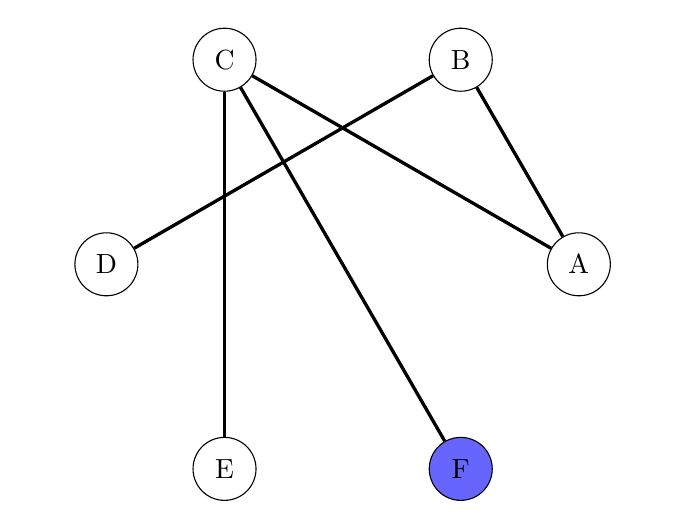
\begin{tikzpicture}
  \filldraw[fill=white!0, draw=none] (-4cm,0) rectangle (4cm, -3cm);
  \node[circle, draw, minimum size=8mm, fill=white] (A) at (0.0:3cm) {A};
  \node[circle, draw, minimum size=8mm, fill=white] (B) at (60.0:3cm) {B};
  \node[circle, draw, minimum size=8mm, fill=white] (C) at (120.0:3cm) {C};
  \node[circle, draw, minimum size=8mm, fill=white] (D) at (180.0:3cm) {D};
  \node[circle, draw, minimum size=8mm, fill=white] (E) at (240.0:3cm) {E};
  \node[circle, draw, minimum size=8mm, fill=blue!60] (F) at (300.0:3cm) {F};
  \draw[black, line width=1.2pt] (A) -- (B);
  \draw[black, line width=1.2pt] (A) -- (C);
  \draw[black, line width=1.2pt] (B) -- (D);
  \draw[black, line width=1.2pt] (C) -- (E);
  \draw[black, line width=1.2pt] (C) -- (F);
\end{tikzpicture}
\end{center}
\noindent\rule{\linewidth}{0.3pt}
\begin{center}
\begin{flushleft}\textbf{Stack}\\[1.75mm]\end{flushleft}
\begin{tikzpicture}
  \filldraw[fill=white!0, draw=none] (0cm,0cm) rectangle (0cm, -1cm);
\end{tikzpicture}
\end{center}
\newpage
% --- Frame 17 ---
\begin{center}\LARGE\textbf{DFS}\\[6mm]\end{center}
\begin{center}
\begin{flushleft}\textbf{Log}\\[1.75mm]\end{flushleft}
\begin{tikzpicture}
  \filldraw[fill=white!0, draw=none] (0,0) rectangle (10cm, -0.25cm);
  \node[anchor=north, align=center, text=black] at (5cm,0) {\texttt{Adding node F's neighbors to stack.}};
\end{tikzpicture}
\end{center}
\noindent\rule{\linewidth}{0.3pt}
\begin{center}
\begin{flushleft}\textbf{Graph}\\[2mm]\end{flushleft}
\begin{tikzpicture}
  \filldraw[fill=white!0, draw=none] (-4cm,0) rectangle (4cm, -3cm);
  \node[circle, draw, minimum size=8mm, fill=white] (A) at (0.0:3cm) {A};
  \node[circle, draw, minimum size=8mm, fill=white] (B) at (60.0:3cm) {B};
  \node[circle, draw, minimum size=8mm, fill=white] (C) at (120.0:3cm) {C};
  \node[circle, draw, minimum size=8mm, fill=white] (D) at (180.0:3cm) {D};
  \node[circle, draw, minimum size=8mm, fill=white] (E) at (240.0:3cm) {E};
  \node[circle, draw, minimum size=8mm, fill=blue!60] (F) at (300.0:3cm) {F};
  \draw[black, line width=1.2pt] (A) -- (B);
  \draw[black, line width=1.2pt] (A) -- (C);
  \draw[black, line width=1.2pt] (B) -- (D);
  \draw[black, line width=1.2pt] (C) -- (E);
  \draw[black, line width=1.2pt] (C) -- (F);
\end{tikzpicture}
\end{center}
\noindent\rule{\linewidth}{0.3pt}
\begin{center}
\begin{flushleft}\textbf{Stack}\\[1.75mm]\end{flushleft}
\begin{tikzpicture}
  \filldraw[fill=white!0, draw=none] (0cm,0cm) rectangle (0cm, -1cm);
\end{tikzpicture}
\end{center}
\newpage
% --- Frame 18 ---
\begin{center}\LARGE\textbf{DFS}\\[6mm]\end{center}
\begin{center}
\begin{flushleft}\textbf{Log}\\[1.75mm]\end{flushleft}
\begin{tikzpicture}
  \filldraw[fill=white!0, draw=none] (0,0) rectangle (10cm, -0.25cm);
  \node[anchor=north, align=center, text=black] at (5cm,0) {\texttt{End of DFS.}};
\end{tikzpicture}
\end{center}
\noindent\rule{\linewidth}{0.3pt}
\begin{center}
\begin{flushleft}\textbf{Graph}\\[2mm]\end{flushleft}
\begin{tikzpicture}
  \filldraw[fill=white!0, draw=none] (-4cm,0) rectangle (4cm, -3cm);
  \node[circle, draw, minimum size=8mm, fill=white] (A) at (0.0:3cm) {A};
  \node[circle, draw, minimum size=8mm, fill=white] (B) at (60.0:3cm) {B};
  \node[circle, draw, minimum size=8mm, fill=white] (C) at (120.0:3cm) {C};
  \node[circle, draw, minimum size=8mm, fill=white] (D) at (180.0:3cm) {D};
  \node[circle, draw, minimum size=8mm, fill=white] (E) at (240.0:3cm) {E};
  \node[circle, draw, minimum size=8mm, fill=white] (F) at (300.0:3cm) {F};
  \draw[black, line width=1.2pt] (A) -- (B);
  \draw[black, line width=1.2pt] (A) -- (C);
  \draw[black, line width=1.2pt] (B) -- (D);
  \draw[black, line width=1.2pt] (C) -- (E);
  \draw[black, line width=1.2pt] (C) -- (F);
\end{tikzpicture}
\end{center}
\noindent\rule{\linewidth}{0.3pt}
\begin{center}
\begin{flushleft}\textbf{Stack}\\[1.75mm]\end{flushleft}
\begin{tikzpicture}
  \filldraw[fill=white!0, draw=none] (0cm,0cm) rectangle (0cm, -1cm);
\end{tikzpicture}
\end{center}
\end{document}